
\documentclass[10pt,a4paper]{article}
\usepackage[latin1]{inputenc}
\usepackage{amsmath}
\usepackage{amsfonts}
\usepackage{amssymb}
\usepackage{xcolor}
\usepackage{textcomp}
\usepackage{graphicx}
\usepackage{capt-of}

\usepackage{listings,,lstautogobble}
\lstset{language=C++,
	basicstyle=\ttfamily,
	keywordstyle=\color{blue}\ttfamily,
	stringstyle=\color{red}\ttfamily,
	commentstyle=\color{purple}\ttfamily,
	morecomment=[l][\color{magenta}]{\#},
	autogobble=true
}
\author{Carter Rhea}
\title{Final Project}
\begin{document}
	\maketitle
	\newpage
	
	\section{Introduction}
	In many elasticity problems involving particle systems held together by surface tension -- such as a particle raft floating upon a think layer of fluid -- the stress strain law exhibits softening. This softening can cause a the general Newton-Raphson solver for nonlinear systems of equations to fail miserably since it cannot traverse the negative slope of the response. Therefore, we must employ differing solvers which can navigate the negative slope region. One of the most popular methods is the arclength method. Instead of using the traditional arclength method, I have opted to use the pseudo arclength method since the pseudo method achieves similar results with considerably less computations. The pseudo arclength method comes about naturally from considering the pythagorean theorem in the space created by the arclength parameter and the displacement parameter. Thus the hypotenuse is the norm of the radius chosen for the arclength method.
		$$||\Delta u||^2 + ||\Delta \lambda||^2 = ||\Delta r||^2 $$
	 Following the approach as laid out by Sandia national lab \cite{arclength}, I sought to employ the linearized arclength constraint equation:
	$$G(u,\lambda) = (u-u_{old})\frac{\partial u}{\partial s}\Big|_{s_i}+(\lambda-\lambda_{old})\frac{\partial \lambda}{\partial s}\Big|_{s_i} - radius$$
	A major practical consideration which I took into account was the initialization of the system.  In concordance with Sandia's arguements I took the following as my initial conditions for the system.		
	$$\frac{\partial \lambda}{\partial s} \Big|_{t_0} = \frac{1}{\sqrt{2}}$$
	$$\frac{\partial u}{\partial \lambda}\Big|_{s_0} \approx \frac{u_1-u_0}{\lambda_1-\lambda_0} $$ 
	$$\frac{\partial u}{\partial s}\Big|_{s_0} = \frac{\partial \lambda}{\partial s}\Big|_{s_0} \frac{u_1-u_0}{\lambda_1-\lambda_0} $$
	$$\Delta s = \frac{\lambda_1-\lambda_0}{\frac{\partial \lambda}{\partial s}\Big|_{s_0}} $$
	
	And thus after initialization we can proceed exactly as expected through subsequent steps by solving simultaneous for the arclength parameter and the other field parameters.
	
	\newpage
	\section{Methods}
	In order to model a solid mechanics problem using the finite element method, my lab uses MOOSE - Multiphysics Object Oriented Simulation Environment. MOOSE is a highly optimized program with contains a number of built-in classes to handle the basics of Tensor Mechanics; however, MOOSE lacks a native solver for the arc-length equation and subsequent implementation. Therefore, it was necessary to write a Scalar Kernel which solved the pseduo-arclength equation (Kernels are the individual classes that get passed to the solver, and they are thought of as individual pieces of physics taken from the weak form of the differential equation).\\
	 The workflow is as follows:
	 \begin{enumerate}
	 	\item Use Auxiliary Kernel to calculate $\Delta u$
	 	\item Postprocess $\Delta u$ in order to determine the average value amongst all elements
	 	\item Calculate $\lambda$ using the Scalar Kernel and the average $\Delta u$.
	 	\item Pass lambda to boundary force and calculate force to be applied at pseudo-time step
	 	\item Solve system $K(d)=\lambda F^{ext} $
	 \end{enumerate}
	In order to impose a softening system, I changed the Youngs Modulus at each iteration which lead to the need to rewrite the kernel which calculated stress and writing a postprocessor to change the Youngs Modulus. 
	\begin{lstlisting}
	PostprocessorValue
	ConstitutiveLaw::getValue()
	{
	if (_Youngs_Modulus*(1-0.1*_t)!=0){
		return _Youngs_Modulus*(1.0-0.1*_t);
	} //end if
	else{
		return _Youngs_Modulus*0.01;
	} //end else
	}
	\end{lstlisting}
	Using this scheme results in the follow stress-strain law (using 10 pseudo-time steps):

	These values were easily obtained from MOOSE using an auxilary kernel and postprocessor to obtain the stress and strain in the x direction along the bottom of a 2d rod undergoing uniaxial tension (see results).
	\newpage
	\section{Results}
	
	\subsection{2 Dimensional Rod}
	
\begin{figure}[h!]
	\centering
	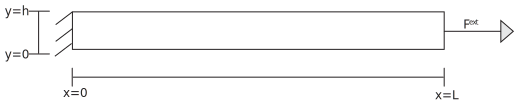
\includegraphics[width=0.7\linewidth]{bar_uniaxial}
	\caption{2D bar undergoing uniaxial tension}
	\label{fig:baruniaxial}
\end{figure}
	The primary benchmark case is a 2 dimensional rod undergoing uniaxial tension in the x-direction. First I applied a constant Youngs Modulus in order to ensure that the physical kernels involving linear elasticity and small strain were properly working. As expected, this statics problem was solved in one step (in contrast to the arc-length method which involves several pseudo-time steps).
	
	
\begin{figure}[h!]
	\centering
	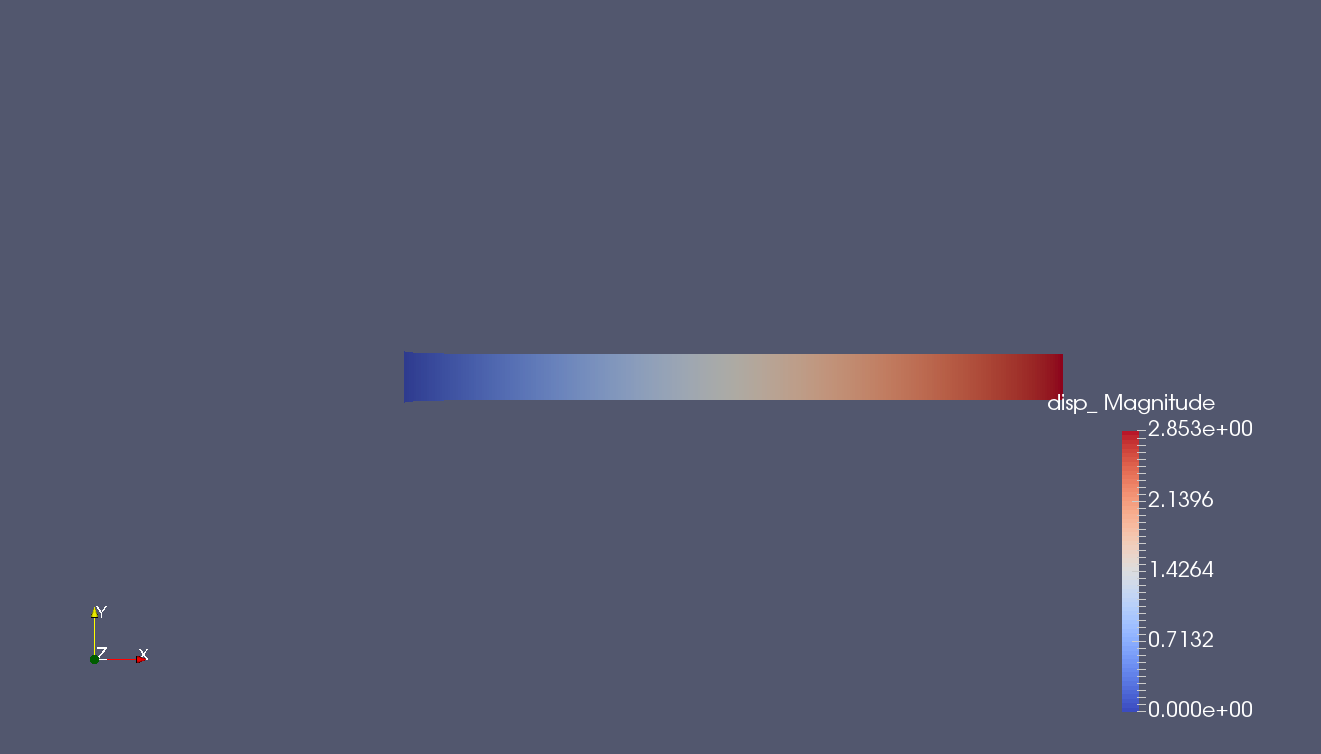
\includegraphics[width=0.7\linewidth]{2d_nolam}
	\caption{A bar undergoing uniaxial tension with 100 elements.}
	\label{fig:2dnolam}
\end{figure}


Comparatively, I was able to implement a pseudo-time stepping mechanism in order to slowly apply a changing force due to the arc-length parameter. In the first test I did not employ softening in the system to ensure that I was achieving comparable results when using the arc-length method. I am able to track the $\lambda$-parameter at each "time-step" and thus determined that 30 pseudo steps were sufficient to achieve a $\lambda$ value of approximately 1.

\begin{figure}[h!]
	\centering
	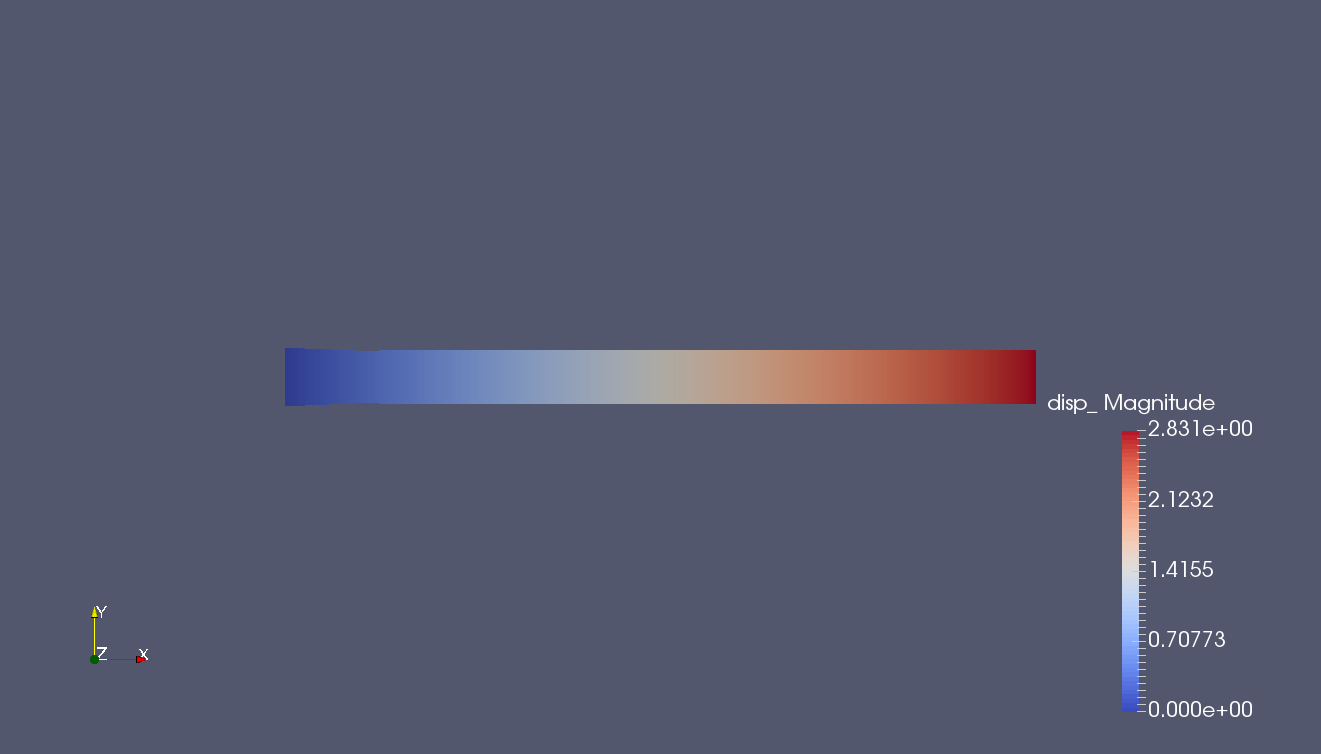
\includegraphics[width=0.7\linewidth]{2d_lam}
	\caption{Bar undergoing uniaxial tension with a loading scheme based on the pseudo arclength paramater. Our final value for $\lambda$ is $9.938527e^{-01} $}
	\label{fig:2dlam}
\end{figure}

\begin{figure}[h!]
	\centering
	\includegraphics[width=0.7\linewidth]{../softening/python/stress_strain}
	\caption{Stress Strain diagram created from changing Youngs Moudlus}
	\label{fig:stressstrain}
\end{figure}

	Hence we can clearly see that we are achieving the same magnitude of displacement. Therefore, feeling confident that the physics and arclength solver were both properly implemented, I added a changing constitutive law through perturbations to the Youngs Modulus. 
	The main indicator that the arclength parameter is properly capturing the softening --besides looking at the stress-strain response of the system-- would come from a decrease in the value which would represent the traversal of the negative slope region of the constitutive law. We can clearly see exactly that by examining the change in lambda.
	
	\begin{figure}[h!]
		\centering
		\begin{minipage}[t]{.58\textwidth}
			\centering
			\vspace{0pt}
			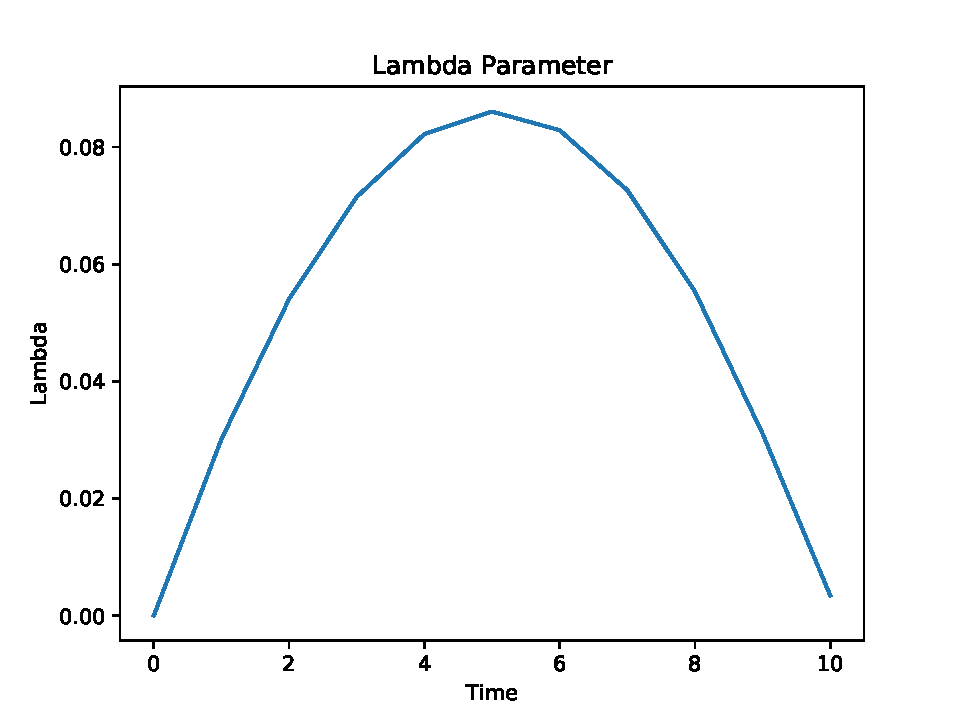
\includegraphics[width=\textwidth]{lambda_CL.pdf}
			\caption{Lambda vs Time}
		\end{minipage}\hfill
		\begin{minipage}[t]{.4\textwidth}
			\centering
			\vspace{0pt}
			\captionof{table}{Lambda values}
				\begin{tabular}{ll}
				\hline
				Time & Lambda \\ \hline
				0    & 0      \\
				1    & 0.030  \\
				2    & 0.054  \\ 
				3    & 0.072  \\
				4    & 0.082  \\
				5    & 0.086  \\
				6    & 0.083  \\
				7    & 0.073  \\
				8    & 0.053  \\
				9    & 0.031  \\
				10   & 0.003 
			\end{tabular}
		\end{minipage}
	\end{figure}
	\subsection{2D Bar Damage}
	After managing to solve problems with softening using the arclength method, I determined to couple the method with damage. Using our labs preconcieved code, I managed to couple damage with the arclength parameter. 
	\subsection{2D Bar Damage with Hole}
	Here we are solving the problem of a bar with a hole centered in the middle. We expect to see the hole morph into an oblong figure due to the stressing, thus inducing vertical stresses into the bar. 
	
	
	
\begin{figure}[h!]
\centering
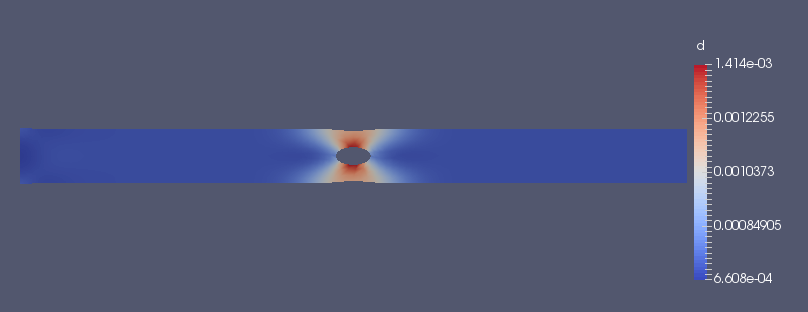
\includegraphics[width=0.7\linewidth]{barwithhole}
\caption{Damage field for bar with hole}
\label{fig:barwithhole}
\end{figure}
	
	\section{Conclusions}
	While the equations for the arclength method are simple and easy to understand, an implementation of the arclength method in any scheme can be wrought with difficulties. In addition to properly formatting the equations in MOOSE, the scheme for linear (and nonlinear) solves had to be considered in order to optimize convergence. Though I ended up opting for using the preconditioned Jaboian-free Newton Krylov method, convergence was not optimal. Finally, with scaling of the damage parameter, I was able to obtain descent convergence for larger problems. Moreover, there was difficulty in properly couping the damage field solves with the arclength solves which normally take two different solving schemes. Hence, I opted for a compromise between the two by relaxing the convergence criterion for the arclength parameter and damage parameter slightly. With the proper finagling of MOOSE, I was able to eventually implement a fully coupled arclength method.
	
	\begin{thebibliography}{9}
		\bibitem{arclength} 
			A. G. Salinger, N. M. Bou-Rabee, R. P. Pawlowski, E. D. Wilkes, E. A.
		Burroughs, R. B. Lehoucq, and L. A. Romero. Sand2002-0396: Loca 1.0
		library of continuation algorithms: Theory and implementation manual.
		Technical report, Sandia National Laboratories, Albuquerque, NM, 2002.
	\end{thebibliography}

	
	
\end{document}